%%%%%%%%%%%%%%%%%%%%%%%%%%%%%%%%%%%%%%%%%%%%%%%%%%%%%%%%%%%%%%%%%%%%%%%%%%%%%%%%%%%%
% Document data
%%%%%%%%%%%%%%%%%%%%%%%%%%%%%%%%%%%%%%%%%%%%%%%%%%%%%%%%%%%%%%%%%%%%%%%%%%%%%%%%%%%%
\documentclass[12pt]{article} %report allows for chapters
%%%%%%%%%%%%%%%%%%%%%%%%%%%%%%%%%%%%%%%%%%%%%%%%%%%%%%%%%%%%%%%%%%%%%%%%%%%%%%%%%%%%
\usepackage{preamble}
\newcommand{\innprod}[2]{\langle #1, #2 \rangle}
\usepackage{subcaption}

\begin{document}

\begin{center}
   \textsc{\large MATH 272, Homework 9, \emph{Solutions}}\\
\end{center}
\vspace{.5cm}

\begin{problem}
	Let $\Psi(x)$ be a complex function with domain $[0,L]$.  Show that multiplication by a global phase $e^{i\theta}$ does not affect the norm of $\Psi(x)$ under the Hermitian (integral) inner product. In more generality, this shows that you cannot fully determine a quantum state -- there will always be an undetermined phase.
\end{problem}
\begin{solution}
	We take the following
	\begin{align*}
		\|e^{i\theta} \Psi\|^2=\innprod{e^{i\theta}\Psi}{e^{i\theta}\Psi} &= \int_0^L \left(e^{i\theta}\Psi(x)\right)\left(e^{i\theta}\Psi(x)\right)^*dx\\
		&= \int_0^L e^{i\theta}e^{-i\theta} \Psi(x)\Psi^*(x)dx\\
		&= \int_0^L \Psi(x)\Psi^*(x)dx\\
		&= \innprod{\Psi}{\Psi}\\
		&= \|\Psi\|^2.
	\end{align*}
\end{solution}

\newpage
\begin{problem}
	Consider the real function $f(x)=1$ on the domain $[0,L]$.
	\begin{enumerate}[(a)]
		\item What is the norm of $f$, $\|f\|$?
		\item Normalize $f(x)$.
		\item Find a nonzero normalized polynomial of degree $\leq 1$ that is orthogonal to $f(x)$.
	\end{enumerate}
\end{problem}
\begin{solution}~
	\begin{enumerate}[(a)]
		\item We compute the norm by
		\begin{align*}
			\|f\| = \sqrt{\innprod{f}{f}} &=\sqrt{ \int_0^L f^2(x)dx}\\
			&=\sqrt{ \int_0^L 1 dx}\\
			&= \sqrt{L}.
		\end{align*}
		\item We can normalize $f$ by letting $c$ be some constant and forcing
		\[
		1=\|cf\| = c^2L.
		\]
		Thus $c=\frac{1}{\sqrt{L}}$.  We can write the normalized function as
		\[
		h(x)=\frac{1}{\sqrt{L}}. 
		\]
		\item Consider an arbitrary polynomial of degree $\leq 1$ by putting $g(x)=ax+b$.  Now, we want this polynomial to be orthogonal to $f(x)$ which means that we want
		\[
		\innprod{f}{g}=0.
		\]
		Let us compute the above
		\begin{align*}
			\innprod{f}{g} &= \int_0^L f(x)g(x)dx\\
			&=\int_0^L ax+bdx\\
			&= \frac{aL^2}{2}+bL\\
			&= \frac{1}{2}L\left(aL+2b\right).
		\end{align*}
		Hence, we can solve for $a$ by
		\[
		0=aL+2b \quad \implies \quad a= -\frac{2b}{L}.
		\]
		Now, $g(x)=-\frac{2b}{L}x+b$.  But, we require $g(x)$ to be normalized as well hence
		\begin{align*}
			1=\innprod{g}{g} &= \int_0^L \left(-\frac{2b}{L}x+b\right)^2dx\\
			&= \frac{b^2L}{3}.
		\end{align*}
		Solving for $b$, we find $b=\sqrt{\frac{3}{L}}$ and hence we have that
		\[
		g(x) = -2\sqrt{\frac{3}{L^3}}x+\sqrt{\frac{3}{L}}..
		\]
	\end{enumerate}
\end{solution}

\newpage
\begin{problem}
	A wavefunction $\Psi(x)$ for a particle in the 1-dimensional box $[0,L]$ could be written as a superposition of normalized states
	\[
	\psi_n(x) = \sqrt{\frac{2}{L}} \sin\left(\frac{n\pi x}{L}\right).
	\]
	That is,
	\[
	\Psi(x) = \sum_{n=1}^\infty a_n \psi_n(x),
	\]
	for some choice of the coefficients $a_n$.
	\begin{enumerate}[(a)]
		\item Let $a_n = \frac{\sqrt{6}}{n\pi}$. Show that $\Psi(x)$ is normalized. \emph{Hint: first, use orthogonality of the states $\psi_n(x)$ to your advantage. Then you will need to know what an infinite series evaluates to. Use a tool like WolframAlpha to evaluate this series.}
		\item Note that we can approximate $\Psi(x)$ by taking a finite sum approximation up to some chosen $N$ by
		\[
			\Psi(x) \approx \sum_{n=1}^N a_n \psi_n(x).
		\]
		Plot the approximation of $\Psi(x)$ for $N=1,5,50,100$.  \emph{Hint: you can modify my Desmos examples.}
		\end{enumerate}
\end{problem}
\begin{solution}
	\begin{enumerate}[(a)]
		\item To see that $\Psi(x)$ is normalized we take
		\begin{align*}
			\innprod{\Psi}{\Psi} &= \innprod{\sum_{n=1}^\infty a_n \psi_n(x)}{\sum_{n=1}^\infty a_n \psi_n(x)}\\
			&= \sum_{n=1}^\infty \|a_n\|^2 \innprod{\psi_n}{\psi_n} &\textrm{by orthogonality of the states}\\
			&= \sum_{n=1}^\infty \frac{6}{n^2 \pi^2}\\
			&= \frac{6}{\pi^2} \sum_{n=1}^\infty \frac{1}{n^2}\\
			&= \frac{6}{\pi^2} \zeta(2)\\
			&= 1.
		\end{align*}
		Note the sum above is the Zeta function we saw in Math 271 and $\zeta(2)$ is a well-known value (that you can find by computing the above sum in, for example, WolframAlpha.
		\item ~
	\begin{figure}[H]
	\centering
		\begin{subfigure}[h]{0.48\textwidth}
			\centering
			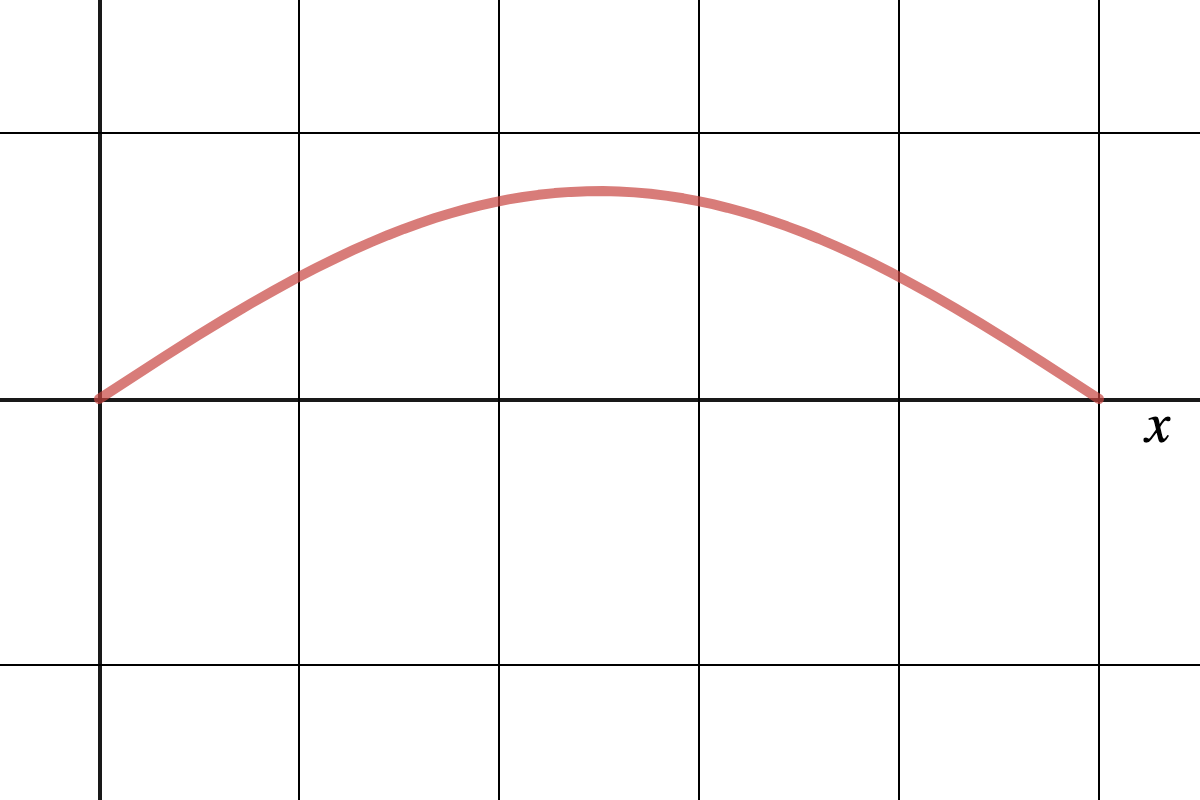
\includegraphics[width=.8\textwidth]{n=1.png}
			\caption{The approximation to $\Psi(x)$ with $N=1$.}
		\end{subfigure}
		~
		\begin{subfigure}[h]{0.48\textwidth}
			\centering
			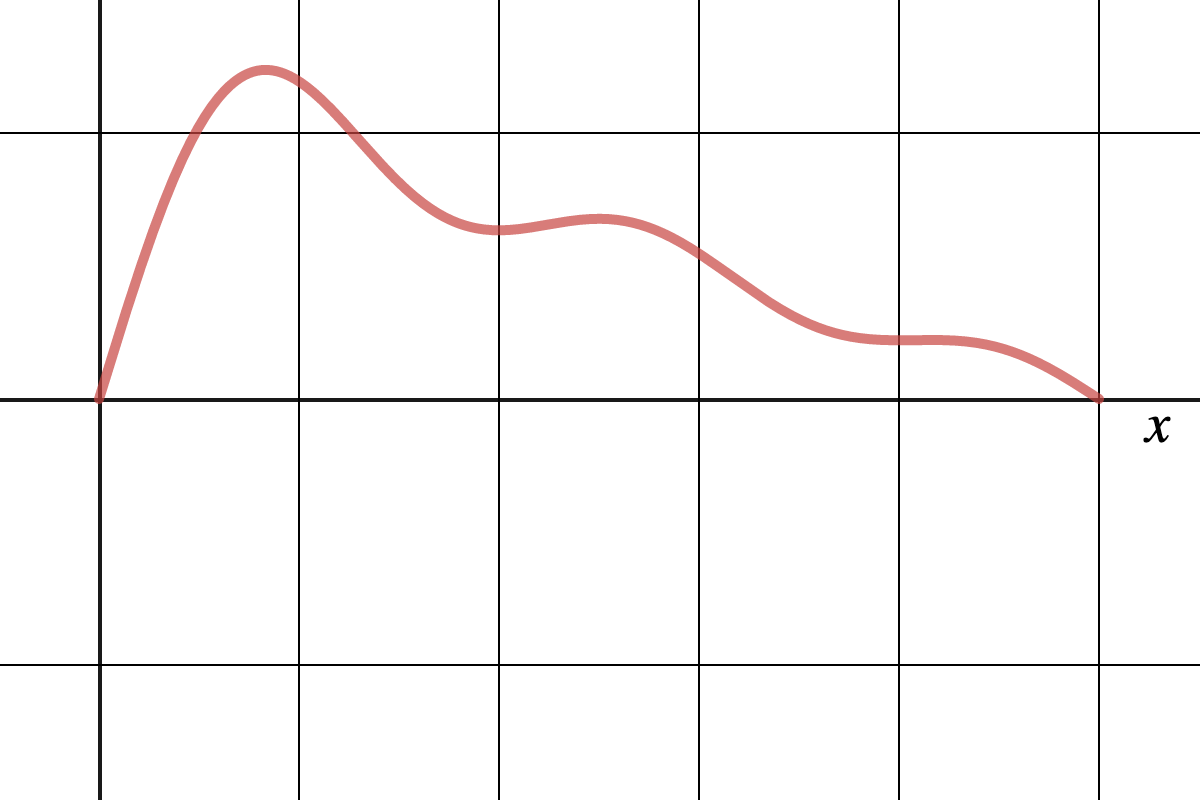
\includegraphics[width=.8\textwidth]{n=5.png}
			\caption{The approximation to $\Psi(x)$ with $N=5$.}
		\end{subfigure}
		\\
		\begin{subfigure}[h]{0.48\textwidth}
			\centering
			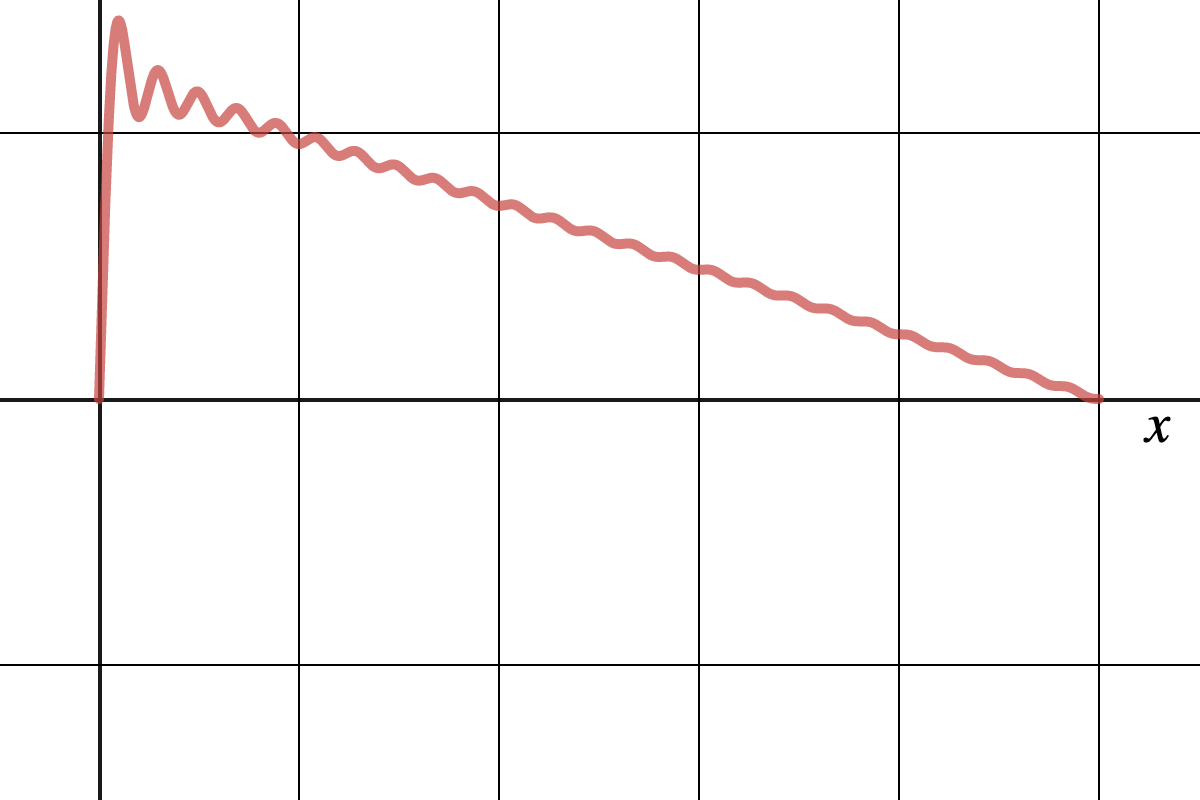
\includegraphics[width=.8\textwidth]{n=50.png}
			\caption{The approximation to $\Psi(x)$ with $N=50$.}
		\end{subfigure}
		~
		\begin{subfigure}[h]{0.48\textwidth}
			\centering
			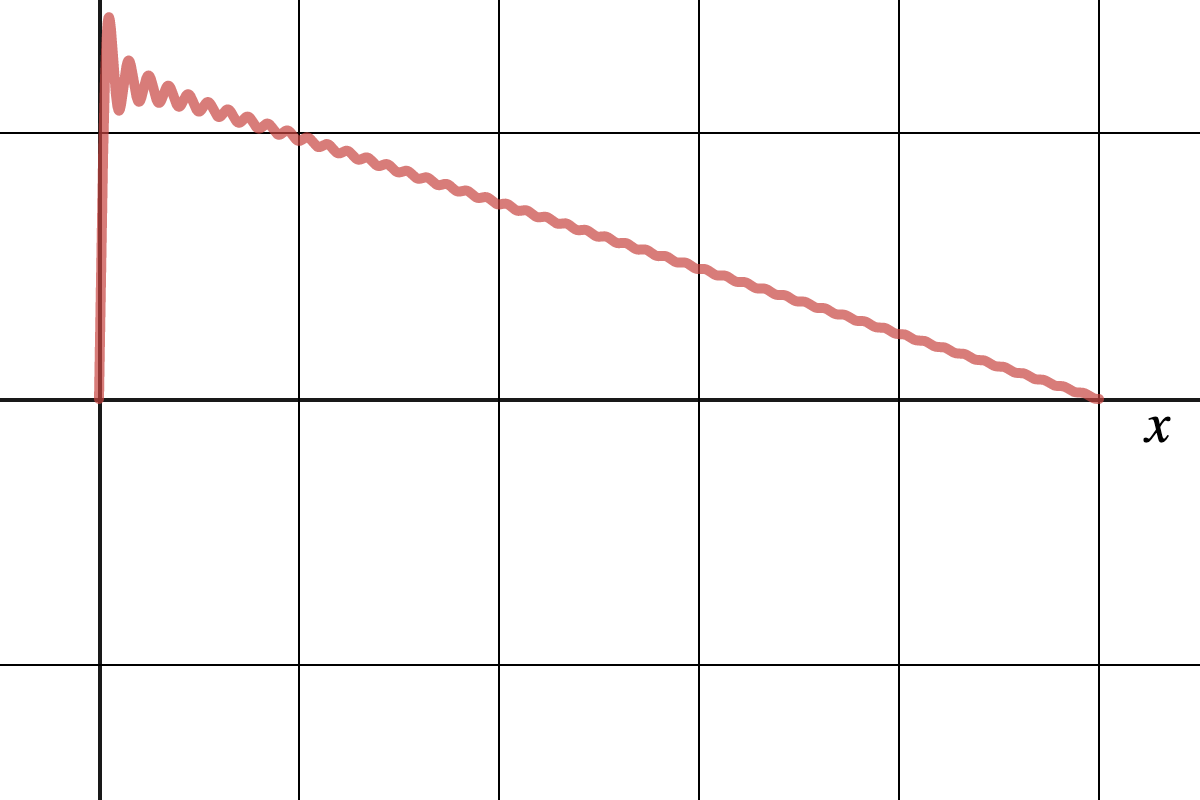
\includegraphics[width=.8\textwidth]{n=100.png}
			\caption{The approximation to $\Psi(x)$ with $N=100$.}
		\end{subfigure}
	\end{figure}
	\end{enumerate}
\end{solution}

\newpage
\begin{problem}
  When making a measurement of the position of the particle, we will use the \emph{position operator} $x$.  This is the same as the variable $x$ in the original problem statement, but it is also an operator!
   \begin{enumerate}[(a)]
   		\item Show that the position operator $x$ is Hermitian.
   		\item We can compute the expected position of a particle with wavefunction $\Psi(x)$ by computing
   		\[
   		\mathbb{E}[x]=\innprod{\Psi}{x\Psi}.
   		\]
   		Let $\Psi(x) = \frac{1}{\sqrt{2}} \psi_1(x) + \frac{1}{\sqrt{2}} \psi_2(x)$, compute $\mathbb{E}[x]$. This value $\mathbb{E}[x]$ tells you where we expect to find the particle on average.
    	\item In fact, any real valued function $V(x)$ of the position operator $x$ is also Hermitian. Make a quick argument on why this must be true.
   	\end{enumerate}
\end{problem}
\begin{solution}
	\begin{enumerate}[(a)]
		\item Let $\Psi(x)$ and $\Phi(x)$ be arbitrary functions.  Then we have
		\begin{align*}
			\innprod{x\Psi}{\Phi} &= \int_0^L x \Psi(x)\Phi^*(x)dx\\
			&= \int_0^L \Psi(x) \left(x \Phi(x)\right)^*dx &\textrm{since $x$ is real valued}\\
			&= \innprod{\Psi}{x\Phi}.
		\end{align*}
		Thus we have that the position operator is Hermitian.
		\item We can compute the expected value by
		\begin{align*}
			\mathbb{E}[x] = \innprod{\Psi}{x\Psi} &= \int_0^L \Psi(x) x^* \Psi(x)dx\\
			&= \int_0^L x\left(\frac{1}{\sqrt{2}}\psi_1(x)+\frac{1}{\sqrt{2}} \psi_2(x)\right)^2dx\\
			&= \int_0^L x \left(\frac{1}{2} \psi_1^2(x) + \psi_1(x)\psi_2(x) + \frac{1}{2} \psi_2^2(x)\right)dx.
		\end{align*}
		This can be split into three separate integrals. First,
		\[
		\int_0^L \frac{x}{2} \psi_1^2(x)dx = \int_0^L \frac{x}{L} \sin^2\left(\frac{\pi x}{L}\right)dx = \frac{L}{4}.
		\]
		Second,
		\[
		\int_0^L x \psi_1(x)\psi_2(x)dx = \int_0^L \frac{2x}{L} \sin\left(\frac{\pi x}{L}\right)\sin\left(\frac{2\pi x}{L}\right)dx = -\frac{16L}{9\pi^2}.
		\]
		Finally,
		\[
		\int_0^L x \psi_2^2(x)dx = \int_0^L \frac{x}{L} \sin^2\left(\frac{2\pi x}{L}\right)dx = \frac{L}{4}.
		\]
		Thus, we can add these all together to get
		\[
		\boxed{\mathbb{E}[x] = \frac{L}{2}-\frac{16L}{9\pi^2}\approx .32L}.
		\]
        \item If $V(x)$ is real valued, then $V^*(x)=V(x)$.  Hence, we have
	\[
	\innprod{V\Psi}{\Phi} = \int_0^L V(x)\Psi(x)\Phi^*(x)dx = \int_0^L \Psi(x)\left(V(x)\Phi(x)\right)^*dx = \innprod{\Psi}{V\Phi}.
	\]
	\end{enumerate}
\end{solution}

\newpage
\begin{problem}
	Another related operator is the \emph{momentum operator} $p = -i\hbar \frac{d}{dx}$. Using integration by parts, show that this operator is Hermitian.
\end{problem}
\begin{solution}
We have
\begin{align*}
	\innprod{p \Psi}{\Phi} &= \int_0^L \left(-i\hbar \frac{d \Psi}{dx}\right)\Phi^*(x)dx\\
	&= \left.-i\hbar \Psi(x)\Phi^*(x)  \right\vert_0^L + \int_0^L i\hbar \Psi(x) \frac{d\Phi^*}{dx}dx & \textrm{by integration by parts}.
\end{align*}
Note now that the boundary conditions require both $\Psi(0)=\Psi(L)=0$ and $\Phi(0)=\Phi(L)=0$, since we are working over the space of solutions to the particle in the 1-dimensional box.  Hence, we have
\begin{align*}
	\innprod{p\Psi}{\Phi} &= \int_0^L i\hbar \Psi(x) \frac{d\Phi^*}{dx}dx\\
	&= \int_0^L \Psi(x)\left(-i\hbar \frac{d\Phi}{dx}\right)^* dx \\
	&= \innprod{\Psi}{p\Phi}.
\end{align*}
Thus, $p$ is Hermitian.
\end{solution}

\newpage
\begin{problem}
	We can always take products, sums, and scalar multiples of operators to build new operators.  For example, in classical physics, we have the kinetic energy
	\[
	T=\frac{1}{2}m \vecv \cdot \vecv,
	\]
	where $\vecv$ is the velocity. In 1-dimension, this reduces to the familiar $\frac{1}{2}mv^2$.  However, we can also rewrite this 1-dimensional equation using the momentum $p=mv$ which gives us the kinetic energy
	\[
	T=\frac{p^2}{2m}.
	\]
	Hence, we can define the quantum \emph{kinetic energy operator}
	\[
	T=\frac{p^2}{2m}.
	\]
	\begin{enumerate}[(a)]
		\item Show that $T = \frac{-\hbar^2}{2m}\frac{d^2}{dx^2}$.
		\item Make a quick argument as to why this kinetic energy operator $T$ is Hermitian.
		\item Again, letting $\Psi(x)=\frac{1}{\sqrt{2}}\psi_1(x)+\frac{1}{\sqrt{2}}\psi_2(x)$, compute $\mathbb{E}[T]$. The expected value $\mathbb{E}[T]$ tells us what the observed energy will be on average. Yet, any time we measure a system we will find that energy must be one of the energy eigenvalues. Thus, for this wave function, this expected value should be the average between $E_1$ and $E_2$ which means that half the time we will measure the energy to be $E_1$ and half the time it will be $E_2$.
	\end{enumerate}	
\end{problem}
\begin{solution}~
	\begin{enumerate}[(a)]
		\item We have $p=-i\hbar \frac{d}{dx}$. Then, we construct $T$ by
		\begin{align*}
		T=\frac{p^2}{2m} &= \frac{\left(-i\hbar \frac{d}{dx}\right)^2}{2m}\\
		&= \frac{-\hbar^2}{2m}\frac{d^2}{dx^2}.
		\end{align*}
		
		\item We have
		\begin{align*}
		\innprod{T\Psi}{\Phi} &= \innprod{\frac{p^2}{2m}\Psi}{\Phi}\\
		&= \innprod{p^2 \Psi}{\frac{1}{2m}\Phi} &\textrm{since $\frac{1}{2m}$ is a real constant}\\
		&= \innprod{p\Psi}{\frac{p}{2m} \Phi} & \textrm{since $p$ is Hermitian}\\
		&= \innprod{\Psi}{\frac{p^2}{2m} \Phi}\\
		&= \innprod{\Psi}{T\Phi}.
		\end{align*}
		Thus, $T$ is Hermitian.
		
		
		\item Now, most of the work has been done for us, and the rest here will be taken care of by orthogonality.  We take
		\begin{align*}
			\innprod{\Psi}{T\Psi} &= \innprod{\frac{1}{\sqrt{2}} \psi_1 + \frac{1}{\sqrt{2}} \psi_2}{\frac{E_1}{\sqrt{2}}\psi_1 + \frac{E_2}{\sqrt{2}}\psi_2}\\
			&= \frac{E_1}{2} \innprod{\psi_1}{\psi_1} + \frac{E_1}{2}\innprod{\psi_2}{\psi_1}+\frac{E_2}{2}\innprod{\psi_1}{\psi_2} + \frac{E_2}{2} \innprod{\psi_2}{\psi_2}\\
			&= \frac{E_1+E_2}{2}.
		\end{align*}
	\end{enumerate}
\end{solution}

\newpage
\begin{problem}
If we are given a potential (energy) $V(x)$ and the kinetic energy $T$, we can take their sum and form the total energy $T+V(x)$ which we call the \emph{Hamiltonian}.  Thus, in the quantum realm, we create the Hamiltonian operator $H$ by
\[
H=T+V(x).
\]
\begin{enumerate}[(a)]
	\item Show that the Hamiltonian operator is Hermitian. \emph{Hint: you have already done the necessary work for this. You just need to combine it and show a few steps here.}
	\item The spectrum of the Hamiltonian tells us the possible energy eigenvalues of a quantum system. Thus, we can compute the spectrum (in this case) by solving the eigenvalue equation
	\[
	H\Psi(x)=E\Psi(x).
	\]
    Explain why the spectrum of $H$ is discrete for the particle in the box problem. \emph{Hint: We have done this exact problem in the notes from Math 271. Feel free to use that!}
\end{enumerate}
\end{problem}
\begin{solution}
	\begin{enumerate}[(a)]
		\item We know that both $T$ and $V(x)$ are Hermitian.  Thus, we take
		\[
		\innprod{(T+V)\Psi}{\Phi} = \innprod{T\Psi}{\Phi}+\innprod{V\Psi}{\Phi} = \innprod{\Psi}{T\Phi}+\innprod{\Psi}{V\Phi} = \innprod{\Psi}{(T+V)\Phi}
		\]
		\item Since $V(x)=0$ in $[0,L]$, we have that
		\[
		H = T = -\frac{\hbar^2}{2m} \frac{d^2}{dx^2}.
		\]
		Hence, we are solving the equation
		\[
		-\frac{\hbar^2}{2m} \frac{d^2}{dx^2}\Psi(x) = E \Psi(x).
		\]
		Let $\omega^2 = \frac{2mE}{\hbar^2}$, and we have
		\[
		\Psi''(x) +\omega^2 \Psi(x) = 0,
		\]
		which is the harmonic oscillator equation.  Thus, our solution is
		\[
		\Psi(x) = C_1 e^{i\omega x}+C_2 e^{-i\omega x}.
		\]
		Now, if we apply the boundary conditions, we have
		\[
		0=\Psi(0)= C_1+C_2,
		\]
		thus $C_1=-C_2$. By Euler's formula, we can take
		\[
		C_1 e^{i\omega x}-C_1 e^{-i \omega x} = C \sin(\omega x).
		\]
		Now, our other boundary condition states
		\[
		0 = \Psi(L) = C\sin(\omega L),
		\]
		Thus we must have $\omega = \frac{n\pi}{L}$ for an integer $n$. Now, this means
		\[
		\frac{2mE}{\hbar^2}=\omega^2 = \frac{n^2\pi^2}{L^2},
		\]
		and we can solve for $E$ to get
		\[
		\boxed{E = \frac{n^2\pi^2\hbar^2}{2mL^2},}
		\]		
		which shows that the spectrum of $H$ is discrete.
	\end{enumerate}
\end{solution}








\end{document}